% Ubah judul dan label berikut sesuai dengan yang diinginkan.
\section{System Design}
\label{sec:systemdesign}

This section describes system design and implementation, it will be divided into two parts: RECORD and PLAY mode.
In RECORD mode, it starts with a human image and then does pose estimation to get human keypoints. After that, converting the angle between 2 keypoints into a servo value
so we can move the robot's servo to mimic human movement and save it for PLAY mode.
On the other hand, in PLAY mode, the input is 2: human image and humanoid robot image. Then, we perform pose estimation for both images. Before doing keypoint normalization,
we have to choose 6 human keypoints based on humanoid robot keypoints. Lastly, we compare those keypoints and get the result.


\subsection{Input Image}
\label{subsec:input-image}

The input image that is fed into both models (human and humanoid robot) is 640x480 pixels with RGB channels. The device for getting the image is the Logitech C920 Webcam. We use OpenCV library to open the camera and capture the image.


\subsection{Human Pose Estimation}
\label{subsec:human-pose-estimation}

Since there are already many pose estimation models for humans out there, we do not need to retrain them and just compare them to find the best model. In order to compare the models, we selected a paper for reference.
So evaluation metrics based on paper and real detection results will be shown in Section \ref{sec:result-and-discussion}, for inference time, we will try in NUC i5. The models that we compare include OpenPose, MediaPipe, and YOLO-pose.
The input for these models is an RGB image and the output is the location of human keypoints.


\subsection{Send Image to Client}
\label{subsec:send-image-to-client}

Our main program uses websites to interact with users because of its flexibility on any platform, the website view can be seen in Figure \ref{fig:websiteview}. So there is a Javascript client and a Python Server that communicate via \emph{socketio}.
The server will send human image to the client so we can adjust our position in the camera. This is done to enable the robot to capture the entire human pose.
\begin{figure}[ht]
  \centering
  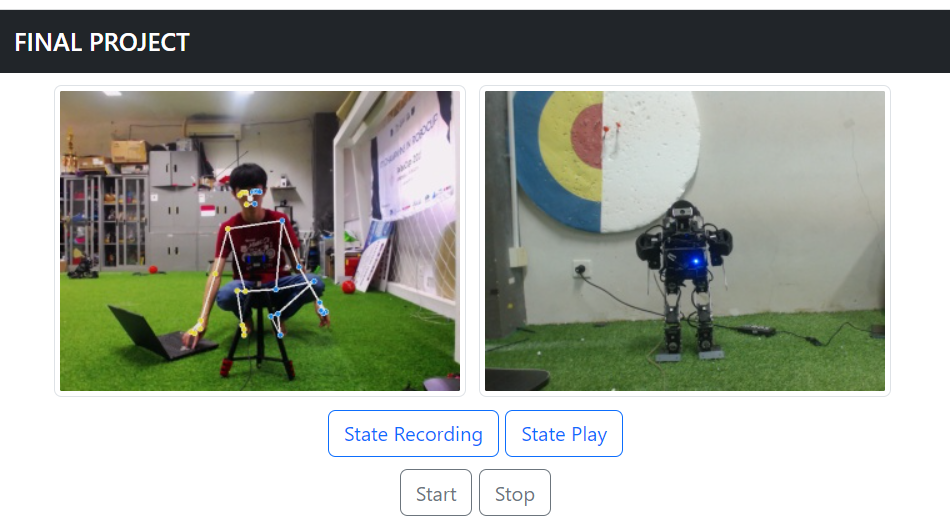
\includegraphics[width=0.48\textwidth]{gambar/web.png}
  \caption{Website View.}
  \label{fig:websiteview}
\end{figure}
The main program is divided into two modes, RECORD mode and PLAY mode. In RECORD mode, a human as a trainer gives a series of movements and will be followed by a humanoid robot, as well as robot saves these movements to use in PLAY mode later.
Meanwhile, in the PLAY mode, the robot acts as a trainer and performs a series of movements according to the movements previously stored in RECORD mode. Human will follow the robot's movement while the robot is also saving both human and robot images and comparing them later.

After getting human's keypoint, the server will visualize the detection result and send it as a buffer to the client.
On the client side, we use ReactJS library. There are four buttons: RECORD, PLAY, START, and STOP button. The RECORD and PLAY button indicates the modes in the main program, while the START and STOP button tell us when the mode is started or stopped.
Apart from that, there are also two images that show human and robot image, actually in RECORD mode there is only one image (human image), while in PLAY mode there are 2 images (human and robot image). 


\subsection{Convert Angle to Servo Value}
\label{subsec:convert-angle-to-servo-value}

This subsection and Subsection \ref{subsec:move-robot-servo} are triggered when the button RECORD and START is pressed on the website, so the client sends this information to the server and it does the calculation. 
To be able to move a robot's upper body like human movement, we need to obtain the angle between 2 keypoint using the \emph{arc tangent} function with the input \emph{\{x,y\}} keypoint coordinate.
Since we use MediaPipe Pose to detect human keypoints, the output is normalized, so we multiplied with the width and height image to get the real pixel value.
Afterward, we divide y with x and input the result to the \emph{arc tangent} function, as shown in Equation \ref{eq:arctan}.
\begin{equation}
  \label{eq:arctan}
  angle = \arctan \left(\frac{Y_2 - Y_1}{X_2 - X_1}\right)
\end{equation}

There are four angles we want to retrieve which are the angles from the shoulder to the elbow (right and left) and also the elbow to wrist (right and left) in order to robot can mimic upper body human movement.
If we look at MediaPipe Pose Landmark, 6 keypoints that become our concern are 11, 12 for shoulders, 13, 14 for elbows, 15, and 16 for wrists. 
We get the right shoulder values by entering landmark 14 as the second argument and landmark 12 as the first argument of the \emph{arc tangent} function. This also applies to get the left shoulder angle value by entering landmarks 13 and 11 respectively. 
It is slightly different to obtain the elbow angles because we want its angle to be relative to the shoulder angle by subtracting its angle from the shoulder angle. We also apply limitations for each angle to keep the servo safe as seen in Table \ref{tb:robot-servos}.

\begin{table}
  \caption{Robot Servos Limitations.}
  \centering
      \begin{tabular}{{ccc}}
      \hline
      \rowcolor[HTML]{C0C0C0}
      \textbf{Joint Angle} & \textbf{Motion} & \textbf{Range (deg)} \\
      \hline
      LShoulderRoll       & Left shoulder joint right and left    & -110 to 30  \\
      RShoulderRoll       & Right shoulder joint right and left   & -30 to 110 \\
      LElbowPitch           & Left Elbow joint front and back       & -120 to 10  \\
      RElbowPitch           & Left Elbow joint front and back       & -10 to 120  \\
      \hline
      \end{tabular}
      \label{tb:robot-servos}
  \end{table}


  \subsection{Move Robot's Servos}
  \label{subsec:move-robot-servo}
  
  The program to move the robot's servos takes the same place as the program for the server. Our main program uses ROS2 with Python language. To be able to run the server and ROS2 program simultaneously, we need a separate thread, so the server program does not block the ROS2.
  In the ROS2 framework, every package has its own functionality. On this occasion, we divide the task to move the robot's servo into 2 packages. The first one is named \emph{motion matching} where the server program and angle conversion to servo value happen, the other one is \emph{tachimawari},
  a package that provides a DYNAMIXEL's joints management library for a ROS 2 project. This package name comes from a Japanese word that means motion. Every package has a node with the package's name like Figure \ref{fig:relation-node-record-mode}.
  We can see this node relationship from rqt graph.
  \begin{figure}[ht]
    \centering
    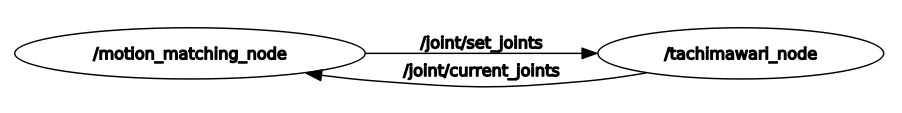
\includegraphics[width=0.48\textwidth]{gambar/rqt_without_akushon.png}
    \caption{Relationship Between Nodes in RECORD Mode.}
    \label{fig:relation-node-record-mode}
  \end{figure}
  
  Each node communicates with each other through a topic. There are 2 topics in RECORD mode, which are \verb|joint/set_joints| and \verb|joint/current_joints|. 
  After getting desired servos angle from the previous section, we just need to publish it to \emph{tachimawari} node and it will move the servos. In the \emph{motion matching} node, there is a publisher that publishes servos angle to \verb|joint/set_joints| topic after the detection process and calculation is done, and also a subscriber in \emph{tachimawari} node that subscribes
  to the same topic which collects the data that is published from the publisher. 
  % \verb|joint/set_joints| topic uses an interface like code snippet \ref{lst:set-joint-msg}, where there are \verb|control_type| variable with type integer and an array with Joint type, each joint consist of id and position like code snippet \ref{lst:joint-msg}.
  % \begin{lstlisting}[
  %   language={},
  %   caption={Joint msg.},
  %   label={lst:joint-msg}
  % ]
  % uint8 id
  % float32 position
  % \end{lstlisting}
  
  % \begin{lstlisting}[
  %   language={},
  %   caption={SetJoints msg.},
  %   label={lst:set-joint-msg}
  % ]
  % int8 control_type 4
  % Joint[] joints
  % \end{lstlisting}
  
  In \verb|tachimawari_node| there is \verb|joint_node| that publishes the current joints every 8ms (it is used in the following section) and has a subscriber that listens to joints that we want to move. 
  In order to move servos to the value that we want, we must enable the torque of all servos first. Then we make a command in array form that contains the servo's id and our desired value or target value (16 bytes) that split into 2 * 8 bytes.
  % For example, our target value is 512 (in binary is equal to \verb|00000010 00000000|), and the message that we send is 2 (\verb|00000010|) and 0 (\verb|00000000|). We can acquire that by performing bitwise AND and bitwise right shift. The bitwise AND operation is performed between the target value and \verb|0xFF|, which is represented as \verb|00000000 11111111| in binary.
  % Since \verb|0xFF| has 0 bits in the higher byte and 1 bits in the lower byte, the result of the operation is the lower byte of the target value. On the other hand, the bitwise right shift operator is used to shift the bits of the target servo 8 positions to the right. Shifting the bits to the right by 8 positions effectively discards the lower byte, leaving only the higher byte in the result.
  % It is the same when we receive the present position from the servo, the servo also sends the data in two bytes (lower and higher) and we need to combine the lower and higher bytes to reconstruct the 16-bit value representing the present position. This can be achieved by performing a left shift operation on the higher byte. Shifting it 8 bits to the left effectively moves it to the higher-order byte position.
  % After that, the bitwise OR operator combines the shifted higher byte with the lower byte. This operation merges the two bytes to form a 16-bit value representing the present position.


\subsection{Save Servos Value}
\label{subsec:save-servo-value}

In the previous section, we discussed a little about the publisher in \emph{tachimawari} package that publishes the value of every current joint of the robot through a \verb|joint/current_joints| topic.
There is also a subscriber in \verb|motion_matching| node that is retrieved that data and a ROS2 timer that is triggered every 0.5 seconds to save the current joints in a JSON format so our robot can move according to the movements exemplified by humans.


\subsection{Humanoid Robot Pose Estimation}
\label{subsec:humanoid-robot-pose-estimation}

This explanation is intended for the RECORD mode. The difference between the PLAY and RECORD modes lies in the number of cameras used.
So there will be two cameras, one camera to record human movement (located on the robot's head) and the other to record robot movement (located from the human side facing the robot), the distance between them approximately 1 - 1.5 meters, as shown in Figure \ref{fig:pose-comparison-side}.
In PLAY mode, the server side sends two images so that we can know and adjust the position of humans and robots in the camera. Due to the large network delay when sending two 320x240 pixel images, when the START button is pressed,
the server does not send the image to client again, the robot plays a series of moves stored in the previous JSON file by communicating via another ROS2 packages, while saving both images. After that, when the STOP button is pressed, the server starts to compare poses between them.
\begin{figure}[ht]
  \centering
  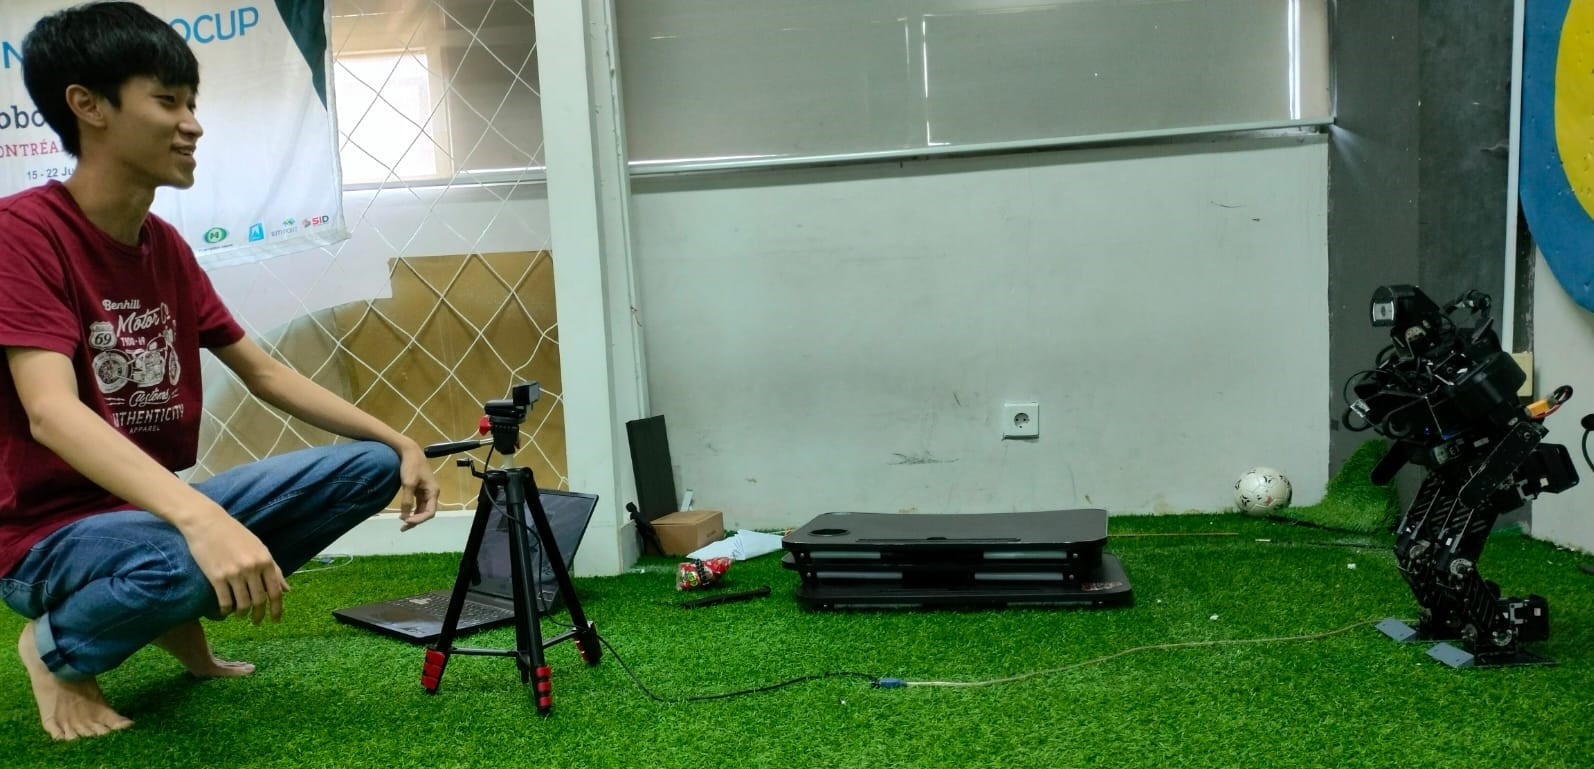
\includegraphics[width=0.47\textwidth]{gambar/pose-comparison.jpeg}
  \caption{Pose Comparison from Side.}
  \label{fig:pose-comparison-side}
\end{figure}

In order to move the servo robot according to the data stored in JSON, a package called \emph{akushon} is needed. \emph{Akushon} is a package related to motion robots. This package name comes from a Japanese word that means action.
Like Subsection \ref{subsec:move-robot-servo}, every package has a node with the package's name and communicates with each other through a topic as shown in Figure \ref{fig:relation-node-play-mode}. There are 3 topics in PLAY mode: \verb|joint/set_joints|, \verb|joint/current_joints| that is used between \verb|akushon_node| and \verb|tachimawari_node| also \verb|motion_matching_node| and \verb|tachimawari_node|,
and \verb|action/run_action| that is used between \verb|akushon_node| and \verb|mo| \verb|tion_matching_node|.
Topic \verb|action/run_action| is used to send pose data in a JSON file from \emph{motion matching} to \emph{akushon} package. In \emph{akushon} package there is an interpolator that loops through every pose in the JSON file, get every value of the servo, and send it to \emph{tachimawari} package.
\begin{figure*}[ht]
  \centering
  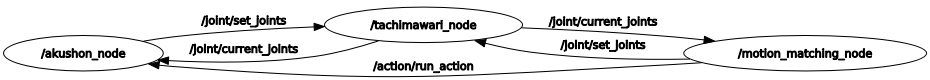
\includegraphics[width=0.8\textwidth]{gambar/rqt_akushon.png}
  \caption{Relationship Between Nodes in PLAY Mode.}
  \label{fig:relation-node-play-mode}
\end{figure*}

Since there are not many pose estimation models for humanoid robots out there yet, we need to retrain them or use transfer learning from the model that supposes to estimate human pose.
Therefore, the three following sections will explain about the steps for training pose estimation on humanoid robot.

\subsection{Make New Dataset}
\label{subsec:make-new-dataset}

This new dataset is a merge of NimbRo's Humanoid Robot Pose dataset and Ichiro's dataset. NimbRo's dataset contains both single and multiple robots to simulate RoboCup's real conditions.
Overall, their dataset has over 1.5k images that come from 23 videos with around 2.3k robot instances. These images include teen and adult-sized robots and contain more than ten different robot types \citep{amini2021}.
However, the robots in Ichiro's dataset are only kid-sized and come in single or maximum two-robot configurations. The images in our dataset come from videos that are taken in our lab. 
Then we split up those videos into multiple images and pick not blurred one.
Before merging, we need to fix NimbRo's dataset format because the width and height were swapped.
After we refine their dataset format and merge them with our dataset, the newly created dataset has approximately 2.1k images.
About 20 percent of the dataset was used for scoring and validating.

When it comes to annotation tools, there are a lot of choices out there including offline and online tools. We have tried some of them like Dataloop, V7labs, or Supervisely which is recommended by NimbRo.
However, when we tried to export the dataset into COCO format, it failed. So, we decided to use a coco-annotator. Regarding the number of keypoints in each robot, we followed NimbRo's dataset.
There are six keypoints including head, trunk, hands, and feet. We stick to that idea because we want to try the model's performance and inference time with fewer keypoints first and if we are confident enough, we will increase the number of keypoints later.


\subsection{Training Pose Estimation Model for Humanoid Robot}
\label{subsec:training-robot}

All of the training processes in this study were primarily conducted on a DGX-A100 server computer and written in the Python programing language.

\subsubsection{NimbRo's Model}
\label{subsubsec:training-nimbro-model}

The hyperparameters that are used to train NimbRo's model followed the description in their paper.
This model is trained using the AdamW optimizer with a learning rate of 10\textsuperscript{-4},
batch size 16, and weight decay of 10\textsuperscript{-4} for the total 200 epochs.
We also use data augmentation that includes random scaling and random translation during training \citep{amini2021}.
We do not use random horizontal flip and random rotation because in our case it will make the training result worse.

The main program for training is already made by them named \emph{main.py} using PyTorch framework, we just need to run it on Jupyter Notebook file or Terminal and adjust the arguments for our needs.
In their script, there is an argument name \verb|config| which it is referred to a file where we store all the hyperparameters, number of epochs, dataset name for training and testing, and many others. 
Another argument tells us about a directory path where we save training results and the dataset takes place.

For computing loss, they use mean square error (MSE) between the predicted heatmaps and the ground truth heatmaps for both keypoints and the limbs.
This loss function directly compare the predicted coordinates of the keypoints with the ground truth coordinates by averaging the squared difference between the predicted and target coordinates.
Finally, the total loss used to train the network is the sum of the keypoint loss and the limb loss \citep{amini2021}.

\subsubsection{YOLO-pose}
\label{subsubsec:training-yolo-pose}

Before jumped into training process, we must change format of our newly dataset from COCO to YOLO. Differ from COCO format, YOLO format gives keypoint confidence or visibility flag 2 for either visible or occluded keypoint
and if it is outside the field of view, the value is set to zero. However, COCO format defines visibility flag as v=0: not labeled, v=1: labeled but not visible, and v=2: labeled and visible. 
Beside keypoint format differences, bounding-box format between them is also different. COCO defines a bounding-box as follow: x (top left), y (top left), width, and height. On the other hand,
bounding-box format in YOLO is: x (center), y (center), width, and height also all of them need to be normalized.

The hyperparameters to train YOLO-pose followed the description in their GitHub named \emph{hyp.pose.yaml}.
We use SGD optimizer with a cosine scheduler. The base learning rate is set to 10\textsuperscript{-2}, batch size 16,
and weight decay of 5\textsuperscript{-4} for total 100 epochs. There are also data augmentation like random scale ([0.5, 1.5]),
random translation [-10, 10], mosaic augmentation with probability 1, and various color augmentations.
It is the same with previous section, the main program for training has been provided using PyTorch framework too, but the program is intended for humans with 17 keypoints.
If we run it directly with our dataset with 6 keypoints, an error will be raised. Therefore, a little bit of code needs to be changed to make the training process can be run.

The overall loss for YOLO-pose is a sum of loss of classification, bounding box, keypoints, and keypoints confidence with its threshold as seen in equation bellow.
The hyper-params that are chosen to balance between losses at different scales are $\lambda_{cls} = 0.5$, $\lambda_{box} = 0.05$, $\lambda_{kpts} = 0.1$, and $\lambda_{kpts_conf} = 0.5$ \citep{maji2022yolopose}.
\begin{equation} \label{eq:overall-loss-yolo}
  \begin{split}
    \mathcal{L}_{total} & = \sum_{s,i,j,k} (\lambda_{cls}\mathcal{L}_{cls} + \lambda_{box}\mathcal{L}_{box} + \lambda_{kpts}\mathcal{L}_{kpts} \\
    & + \lambda_{kpts_conf}\mathcal{L}_{kpts_conf})
  \end{split}
\end{equation}

\subsubsection{Keypoint RCNN}
\label{subsubsec:training-rcnn}

The Keypoint RCNN training is done on Jupyter Notebook directly using the PyTorch framework as well.
The training process starts with loading our dataset and specifying the augmentation technique we are using. We use \emph{albumentations} library from Python for augmenting our dataset.
We apply random brightness, contrast, and rotation.
Before we declare RCNN model using torchvision library, we need anchors that will be an input argument. 
By default, the \emph{AnchorGenerator} class in PyTorch has 3 different sizes (128, 256, 512) and 3 different aspect ratios (0.5, 1.0, 2.0).
We have extended those parameters, \verb|sizes| to (32, 64, 128, 256, 512) which means that anchor boxes with different base sizes will be generated.
By combining different base sizes and aspect ratios, the anchor generator can produce a diverse set of anchor boxes.
Note that, \verb|num classes| argument is set to two because the first class is background and object is the second class.
In this training, we use SGD optimizer with learning rate 10\textsuperscript{-3}, batch size 3, and weight decay of 5\textsuperscript{-4} for 50 epochs.

The total loss for Keypoint RCNN is a sum of loss for classification, bounding box, and keypoints as seen in Equation \ref{eq:overall-loss-rcnn}.
Keypoint RCNN use Cross-Entropy Loss to compute classification loss and keypoints loss, also smooth L1 loss for bounding-box. 
\begin{equation}
  \label{eq:overall-loss-rcnn}
  \mathcal{L}_{total} = \sum (\mathcal{L}_{cls} + \mathcal{L}_{box} + \mathcal{L}_{kpts})
\end{equation}

\subsection{Finding the Best Model for Humanoid Robot Pose Estimation}
\label{subsec:finding-best-model-humanoid-robot}

After retraining 3 models on Subsection \ref{subsec:training-robot}, we try to find the best one for our case. We compare them based on \emph{AP} (Average Precision), \emph{AR} (Average Recall),
real detection result, and inference time on devices with limited computing capabilities (e.g. NUC i5).
The comparison table and real detection result of those models are in Section \ref{sec:result-and-discussion}.
To know the time that it takes for the model to do the detection, we just need to subtract the time before and after the model does keypoint detection.
We also attempt converting our models from PyTorch Model to OpenVINO in order to speed up the time inference. Before that, we convert it to ONNX first.

\subsection{Choose Six Keypoints based on Humanoid Robot Keypoints}
\label{subsec:choose-keypoints}

The difference in numbers between human keypoints and robot keypoints makes us have to choose certain human's keypoints in order to make a comparison between them.
Based on the results after testing, we chose Mediapipe for human and Keypoint RCNN for robot. Mediapipe provides 33 landmark keypoints for human and Keypoint RCNN only provides 6 keypoints.
Therefore, we need to choose 6 from 33 human keypoint.
First, we get all 33 keypoints. Then calculate the keypoint we want, such as the head keypoint which is located between the right and left eye.
To obtain the eye landmarks, we can index according to the MediaPipe Landmark, where the left eye is index 2 and the right eye is index 5. This also applies to other landmarks.
The keypoint for the hands and feet is simply to select the wrists and ankles.
Lastly, the trunk keypoint is located between the shoulder and hip keypoint.
After all of the computation, we arrange all keypoints in a single array and return it.


\subsection{Keypoint Normalization}
\label{subsec:keypoint-normalization}

When we think about the problem, we see that there are many uncertainties to be addressed. For example, human and humanoid robot can differ in height, body shape, and location within an image: one subject (human or robot) may have been nearby the camera,
while another may have been in the distance. In order to get an accurate outcome, each of these issues must be resolved.
After choosing the keypoints, the model output for both human and robot is the coordinates of 6 keypoints. This information can be used to create a new keypoint coordinates starting from (0,0) in the image. This solves the problem of the subject appearing in different parts of the picture.
We further normalized the resulting keypoints coordinates by performing L2 normalization in order to transform it into a unit vector.
This means we are ignoring the size of the picture, but keeping in account the direction of the vector, created by the pose inside of that image.


\subsection{Comparing Human Keypoints and Robot Keypoints}
\label{subsec:comparing-keypoints}

Now that we have standardized the pose vectors, it is time to choose a similarity measure. We chose cosine similarity and performing a few calculations detailed below to arrive at a Euclidean distance that can be interpreted as a cosine distance.
The cosine similarity ranges from -1 to 1. The cosine distance, on the other hand, is a dissimilarity measure that ranges from 0 to 2.
Using Equation \ref{eq:euclideandistance} scales the values to the range of 0 to 2, making it easier to interpret the results. A larger value implies a greater dissimilarity between poses. In that equation, Fxy and Gxy are two pose vectors to be compared after L2 normalization. Moreover, Fxy and Gxy contain only x and y positions for each of the 6 keypoints, it does not include confidence scores.
\begin{equation} 
  \label{eq:cosinesimilarity}
  cosineSimilarity(x,y) = \frac{x \cdot y}{|x||y|}
\end{equation}

\begin{equation}
  \label{eq:euclideandistance}
  D(F_{xy}, G_{xy}) = \sqrt{2 * (1 - cosineSimilarity(F_{xy}, G_{xy}))}
\end{equation}


\subsection{Pose Similarity Result}
\label{subsec:pose-similarity-result}

The result of pose similarity is in percentages with a range of 0 to 100. A higher score indicates a more similar position between the human and robot, and vice versa.
In order to get it, we multiply the cosine distance result from Section \ref{subsec:comparing-keypoints} by 100 and subtract the result from 100.
After getting each result of pose similarity, we take a mean and display it in the left top video. This video will be generated after detecting and comparing all poses.